\documentclass[twocolumn]{jsarticle}
%
\usepackage{amsmath,amssymb}
\usepackage{bm}
\usepackage{graphicx}
\usepackage{ascmac}
\usepackage{subfigure}
\usepackage{multicol}
\usepackage{setspace}
%
\setlength{\textwidth}{\fullwidth}
\setlength{\textheight}{39\baselineskip}
\addtolength{\textheight}{\topskip}
\setlength{\voffset}{-0.5in}
\setlength{\headsep}{0.3in}
%
\newcommand{\divergence}{\mathrm{div}\,}  %ダイバージェンス
\newcommand{\grad}{\mathrm{grad}\,}  %グラディエント
\newcommand{\rot}{\mathrm{rot}\,}  %ローテーション
\renewcommand{\baselinestretch}{1.3}
\renewcommand{\figurename}{Fig.}
\renewcommand{\tablename}{Table.}

\newcommand{\bi}{\bfseries\itshape}
\newcommand{\bq}{\begin{equation}}
\newcommand{\eq}{\end{equation}}
\newcommand{\bn}{\vspace{-2mm}\begin{eqnarray}}
\newcommand{\en}{\vspace{-2mm}\end{eqnarray}}
\newcommand{\ba}{\begin{array}}
\newcommand{\ea}{\end{array}}
\newcommand{\lt}{\left}
\newcommand{\rt}{\right}
\newcommand{\bc}{\begin{center}}                            %%% 中央揃え
\newcommand{\ec}{\end{center}}
\newcommand{\bfr}{\begin{flushright}}                       %%% 右揃え
\newcommand{\efr}{\end{flushright}}
\newcommand{\beqa}{\begin{eqnarray}}                        %%% 数式
\newcommand{\eeqa}{\end{eqnarray}}
\newcommand{\ben}{\begin{enumerate}}                        %%% ラベル  1. → (a) → .
\newcommand{\een}{\end{enumerate}}
\newcommand{\bib}{\begin{itembox}}                          %%% 枠
\newcommand{\eib}{\end{itembox}}
\newcommand{\nn}{\nonumber}                                 %%% 式番号表示なし
\newcommand{\lw}[1]{\smash{\lower2.0ex\hbox{#1}}}           %%%
\newcommand{\ds}{\displaystyle}                             %%% ディスプレイスタイル
\newcommand{\unsc}[1]{_{\scriptscriptstyle {#1}}}           %%% 下添え字を \scriptscriptstyle で
\newcommand{\upsc}[1]{^{\scriptscriptstyle {#1}}}           %%% 上添え字を \scriptscriptstyle で
\newcommand{\sq}{\upsc{2}}                                  %%% 二乗
\newcommand{\T}{\upsc{\rm{T}}}                              %%% 転置記号
\newcommand{\inv}{\upsc{-1}}                                %%% 逆行列
\newcommand{\msc}[1]{\mathscr{#1}}                          %%% 花文字
\newcommand{\ut}{\unsc{t}}                                  %%%
\newcommand{\uto}{\unsc{t+1}}                               %%%
\newcommand{\us}{\unsc{s}}                                  %%%
\newcommand{\uz}{\unsc{0}}                                  %%%
\newcommand{\Dt}{\Delta t}                                  %%%
\newcommand{\coef}[1]{\frac{\sigma\unsc{w,j}\sq}{2\alpha\unsc{j}\upsc{#1}}}
\newcommand{\ex}[1]{e\upsc{-#1\alpha\unsc{j}\Dt}}
\newcommand{\bmat}{\lt[ \ba}                                %%% 行列表示 [ ]
\newcommand{\emat}{\ea \rt]}
\newcommand{\reff}[1]{(\ref{#1}) 式}
\newcommand{\tripo}{\raisebox{.2ex}{.}\raisebox{1.2ex}{.}\raisebox{.2ex}{.}}
\newcommand{\maru}[1]{{\ooalign{\hfill\raisebox{-0.2ex}     %%% 文字を丸で囲む
           {$\scriptsize#1$}\hfill\crcr$\bigcirc$}}}

\begin{document}
\twocolumn[
\begin{screen}
\begin{flushleft}
融合情報学輪講資料\hspace{\fill}2013/06/14
\end{flushleft}
\begin{center}
{\Large  Webアクセススピード改善に関する研究動向 \\
Recent Trend of Improving Web Access Speed}
\end{center}
\begin{flushleft}
工学系研究科 電気系工学専攻 関谷研究室\hspace{\fill}修士課程1年 37-136482 藤居 翔吾
\end{flushleft}
\end{screen}
]

\begin{bfseries}
\begin{itshape}
Abstract-
\end{itshape}
Web access is

\begin{itshape}
Index-
\end{itshape}
\end{bfseries}
\section{Introduction}
近年のWebページは, 静的なテキストや静止画像だけでなく, 動的な映像やアニメーション, CG, 音声を利用し, インタラクティブな表現が可能になっている.
そのような需要により, IPトラヒックの量が増加傾向にある.
Fig{\ref{}}に, Ciscoによる, IPトラヒックの予測データを示す.
このグラフから分かるように, 今後も比例的にトラヒックが増加する事が分かる.
%\begin{figure}[htbp]
%    \begin{center}
%        \includegraphics[width=5cm]{eps/IPtraffic.eps}
%    \end{center}
%\end{figure}
同様にモバイルに関しても,モバイルトラヒックの予測を行っており, Fig{\ref{}}に示す.
%\begin{figure}[htbp]
%    \begin{center}
%        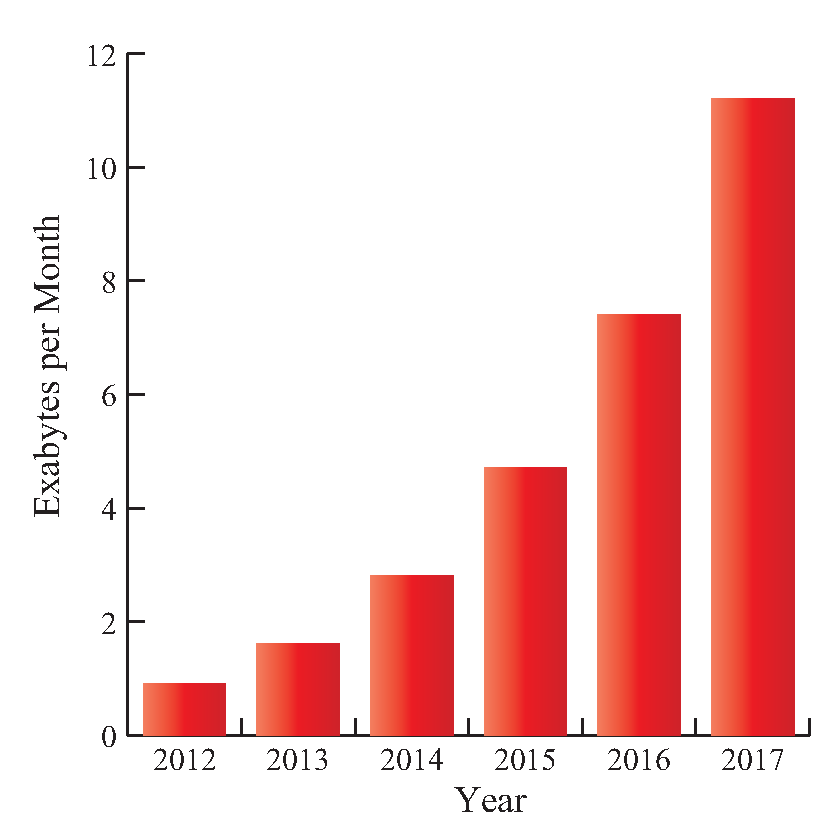
\includegraphics[width=5cm]{eps/mobile_traffic.eps}
%    \end{center}
%\end{figure}
ように トラヒック量が比例的ではなく, 指数関数的に増加している事が分かる.
このことから, 今後, 爆発的な増加が目立つモバイルにおいても, 既存のイーサネットにおいても, クライアントとサーバ間で扱うデータの量は増加していく.
また, それにより, クライアント側で処理しなければならないコードの量も, 増えてくる.
さらに, リッチコンテンツの台頭により, クライアント側で, より複雑なレンダリングを要求される.
このような傾向から, ウェブアクセスの高速化技術のニーズが高まっている.

一般に, ウェブアクセスの改善には, 以下のような4つのアプローチがある.
\begin{itemize}
  \item 通信性能の向上
  \item レンダリング性能の向上
  \item ユーザーエクスペリエンスの向上
  \item コード実行の最適化
\end{itemize}
これまで, 多くのウェブアクセスの改善に関する研究がこれらのアプローチによって行われてきた.
特に通信性能の向上に対する研究によって, モバイルネットワークにおけるデータ帯域が飛躍的に上昇している.
Table\ref{}に, 世代ごとの移動通信システムの転送速度の変遷を示す.
4G回線においては, ピーク時100~300[Mbps]の速さで通信する事が可能になった.
\begin{table}[htb]
    \caption{Transition of mobile network}
  \begin{tabular}{|c||c|c|} \hline
     & 1G & 2G \\ \hline \hline
     Period & 1980s & 1990s \\ \hline
     Srandard & AMPS &\shortstack{\\ PDC \\ GSM} \\
     \hline
     Down rate & -8kbps & -64kbps \\ \hline \hline
     & 3G & 4G \\ \hline \hline
     Period & 2000s & 2010s \\ \hline
     Srandard &  \shortstack{\\ W-CDMA \\
     CDMA-2000}&\shortstack{\\ LTE-Advanced \\ WIMAX2}
     \\
     \hline
     Down rate  & -200kbps & 50Mbps-1Gbps \\ \hline
  \end{tabular}
\end{table}

このような背景から, モバイルネットワークにおける帯域幅の効率的な利用による, ウェブアクセス高速化の要求が高まってきた.
通信において, ウェブアクセスの性能は, レスポンス時間によって決定される.
レスポンス時間とは, ユーザーによるページの送信要求から, 対象のデバイスで全てのページのレンダリング終了までの時間である.
本稿では, 2章で, 既存のウェブアクセス処理の流れと, それに基づく高速化に対するアプローチを示す.
3章では, ページローディング時間改善に対する具体的な手法である, HTTPパイプライン, SCTP(Stream Control Transmission
Protocol), SPDYで使われている高速化技術を示す.
4章では,HTTPパイプライン, SCTP, SPDYの評価結果を示す.
5章では, SPDYを応用したウェブアクセス高速化技術を紹介し, ウェブにおけるレスポンス向上に対する道筋を示す.
最後に, 6章では, 本稿で取り扱ったウェブアクセス高速化技術やその考え方をまとめる.

\section{既存のウェブアクセス処理の流れ}


\end{document}